\ESKDappendix{обязательное}{Уравнения используемых элементарных траекторий}\label{app_elementary_trajectories}

В~работе используются траектории в виде отрезка прямой и дуги окружности с центральным углом, на который она опирается, меньшим~$\pi$, параметризованные временем, (см.~рисунок~\ref{img_elem_trajs}) и описываемые следующими выражениями ($v$~--- желаемая скорость движения по траектории, $t_{end}$~--- время, необходимое для прохождения всей траектории):
\begin{itemize}
    \item отрезок прямой:
    \begin{gather}
        \left\{
        \begin{aligned}
            & x_{r}(t) = x_0 + v_x t, \\
            & y_{r}(t) = y_0 + v_y t,
        \end{aligned}
        \right.
        \qquad
        \left\{
        \begin{aligned}
            & \dot{x}_{r}(t) = v_x, \\
            & \dot{y}_{r}(t) = v_y,
        \end{aligned}
        \right.
        \qquad
        \left\{
        \begin{aligned}
            & \ddot{x}_{r}(t) = 0, \\
            & \ddot{y}_{r}(t) = 0,
        \end{aligned}
        \right.
        \\[0.2cm]
        \gamma = \atan2(y_1 - y_0,\ x_1 - x_0),
        \qquad
        v_x = v \cos \gamma,
        \qquad
        v_y = v \sin \gamma,
        \\[0.2cm]
        t_{end} = \cfrac{\sqrt{(y_1 - y_0)^2 + (x_1 - x_0)^2}}{v} ;
    \end{gather}
    \begin{figure}[h]
        \centering
        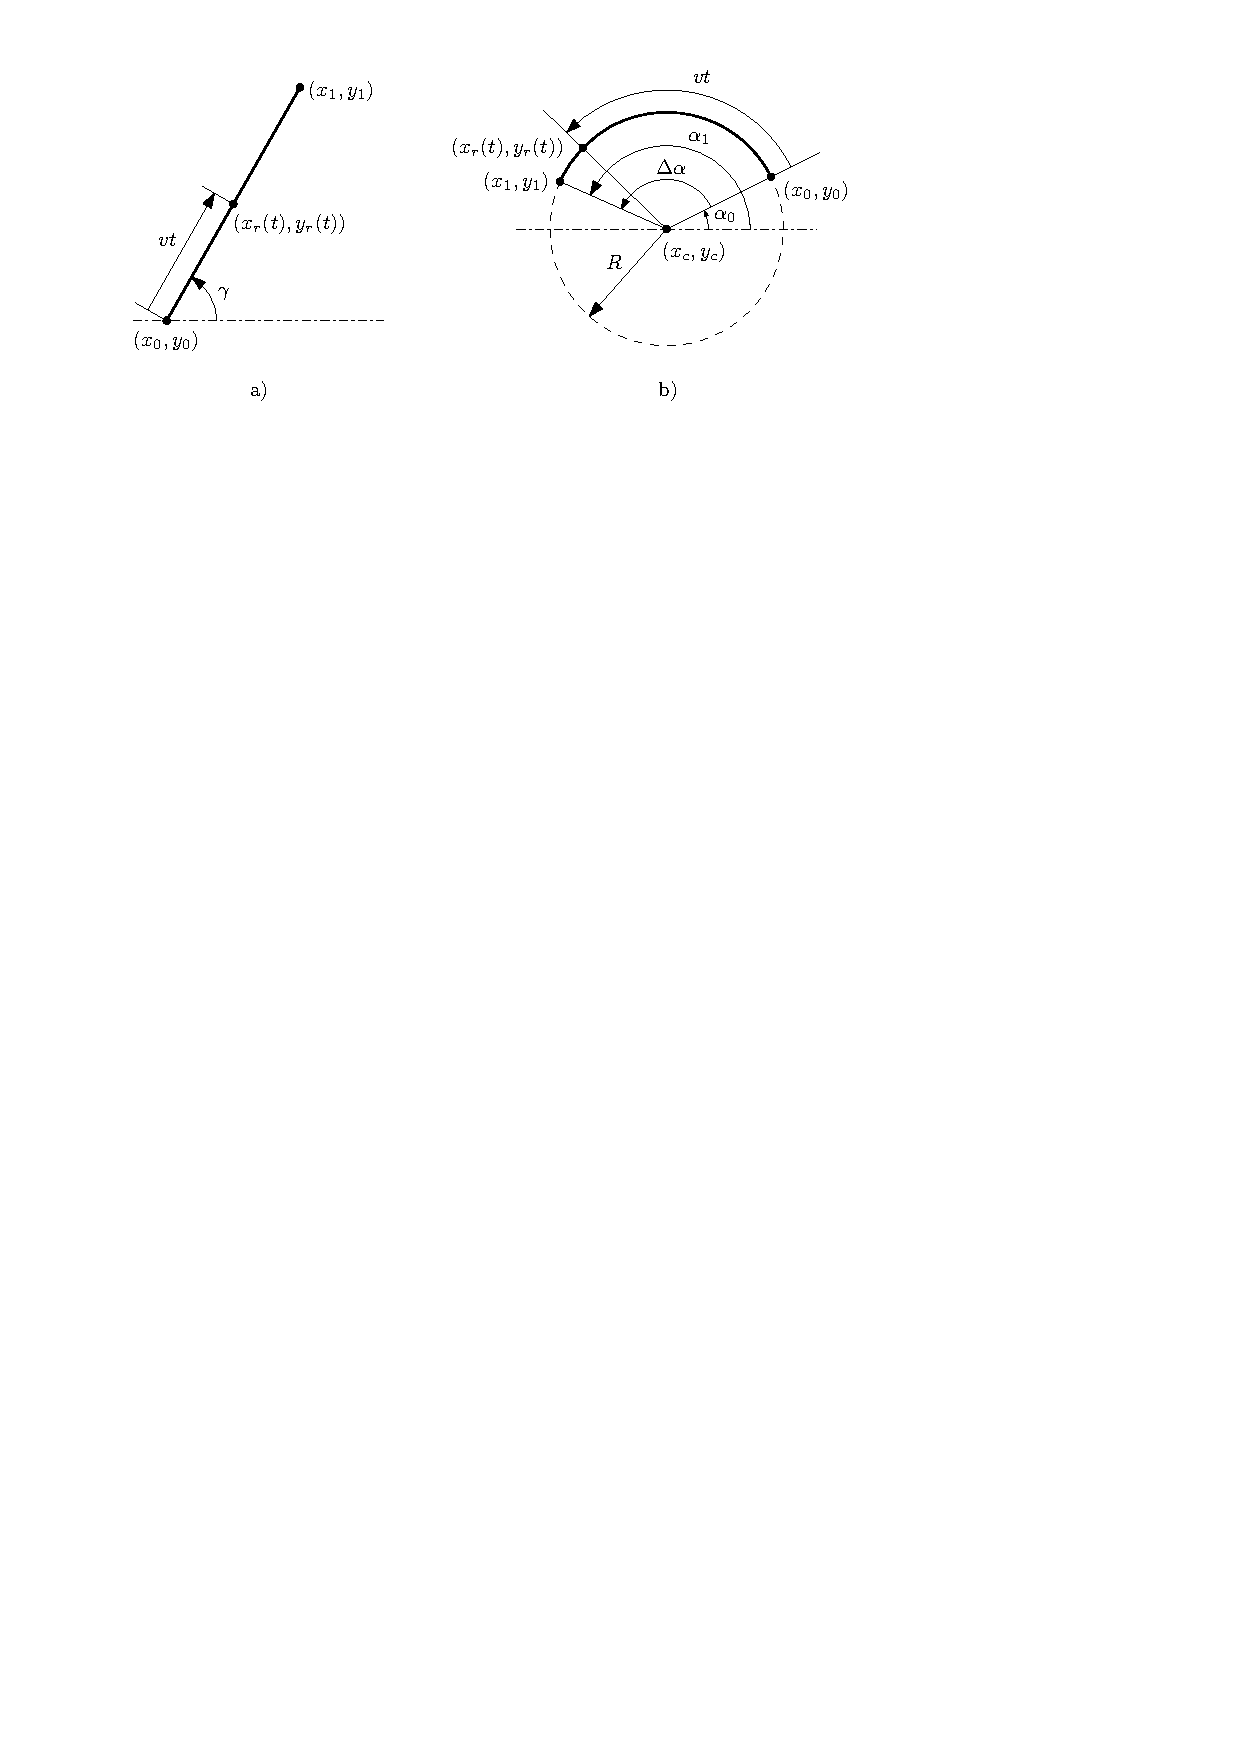
\includegraphics[width=0.9\textwidth]{elem_trajs.pdf}
        \caption{Рассматриваемые траектории: a~--- отрезок прямой, b~--- дуга окружности.}
        \label{img_elem_trajs}
    \end{figure}
    \item окружность:
    \begin{gather}
         \left\{
         \begin{aligned}
             & x_{r}(t) = x_c + R \cos \alpha, \\
             & y_{r}(t) = y_c + R \sin \alpha,
         \end{aligned}
         \right.
         \qquad
         \left\{
         \begin{aligned}
             & \dot{x}_{r}(t) = -R \omega \sin \alpha, \\
             & \dot{y}_{r}(t) = R \omega \cos \alpha,
         \end{aligned}
         \right.
         \qquad
         \left\{
         \begin{aligned}
             & \ddot{x}_{r}(t) = -R \omega^2 \cos \alpha, \\
             & \ddot{y}_{r}(t) = -R \omega^2 \sin \alpha,
         \end{aligned}
         \right.
        \\[0.2cm]
        R = \sqrt{(x_0 - x_c)^2 + (y_0 - y_c)^2},
        \qquad
        \alpha_0 = \atan2 \bigl( y_0 - y_c,\ x_0 - x_c \bigr),
        \\[0.2cm]
        \alpha = \alpha_0 + \omega t,
        \qquad
        \alpha_1 = \atan2 \bigl( y_1 - y_c,\ x_1 - x_c \bigr),
        \qquad
        \omega = \frac{v}{R} \sign(\Delta\alpha),
        \\[0.2cm]
        t_{end} = \cfrac{|\Delta\alpha|}{\omega},
        \qquad
        \Delta\alpha =
        \begin{cases}
            \alpha_1 - \alpha_0, & \alpha_1 - \alpha_0 \in (-\pi; \pi), \\
            \alpha_1 - \alpha_0 - 2\pi, & \alpha_1 - \alpha_0 > \pi, \\
            \alpha_1 - \alpha_0 + 2\pi, & \alpha_1 - \alpha_0 < -\pi \ldotp
        \end{cases}
    \end{gather}
\end{itemize}

